\subsection{Taylor 급수}\label{ch:4-1}
Taylor 정리(Taylor theorem)와 이에 관련된 Taylor급수는 수치해법의 학습에 매우 중요한 가치를 갖는다. \textbf{Taylor 급수는 함수값 및 그의 도함수값들을 사용하여 예측하는 방법을 제공한다.}
\\
\rule{\textwidth}{0.1pt}
%\begin{minipage}
만일 함수 $f$와 그것의 처음 $(n+1)$차까지의 미분이 $a$와 $x$를 포함하는 구간에서 연속적이라면, $x$에서의 함수값은 다음과 같이 주어진다.
\begin{equation}
f(x)=f(a)+f'(a)(x-a)+\frac{f''(a)}{2!}(x-a)^2+\frac{f^{(3)}(a)}{3!}(x-a)^3 +\cdots +\frac{f^{(n)}}{n!}(x-a)^n+R_{n}
\end{equation}

여기서 나머지(remainder) $R_n$은 다음과 같이 정의된다.
\begin{equation}
R_n = \int_{a}^{x} \frac{(x-t)^n}{n!}f^{(n+1)}(t)dt
\end{equation}
여기서 $t$는 모조변수(dummy variable)이다.\\
\rule{\textwidth}{0.1pt}

%\end{minipage}
Taylor 급수를 통해 통찰력을 얻는 유용한 방법은 항을 추가해보면서 급수를 구성해보는 방법이다. 

Taylor급수에서 $x$를 이전 함수값에 의한 새로운 위치 즉 $x_{i+1}$, 그리고 $a$를 이전 함수값의 위치 $x_{i}$로 생각해보자.

\begin{equation}
f(x_{i+1})=f(x_{i})+f'(x_{i})(x_{i+1}-x_{i})+\frac{f''(x_{i})}{2!}(x_{i+1}-x_{i})^2+\frac{f^{(3)}(x_{i})}{3!}(x_{i+1}-x_{i})^3 +\cdots +\frac{f^{(n)}}{n!}(x_{i+1}-x_{i})^n+R_{n}
\label{eq:4-7}
\end{equation}

\begin{itemize}
\item 0차근사(zero-order approximation) :  \framebox{$f(x_{i+1})\cong f(x_{i})$} \\ 새로운 위치에서의 함수값은 이전의 위치에서의 \textbf{함수값}과 같다.
\item 1차근사(first order approximation) : \framebox{$f(x_{i+1})\cong f(x_{i})+f'(x_{i})(x_{i+1}-x_{i})$} \\ 이전의 위치에서의 \textbf{함수값}과 \textbf{기울기} $f'(x_{i})$에 이전위치 $x_{i}$와 현재 위치 $x_{i+1}$사이의 \textbf{거리}가 곱해져서 얻어진다. 즉 이 표현은 직선의 형태를 가지며, $x_{i}$와 $x_{i+1}$사이의 구간에서 함수의 증가나 감소를 예측할 수 있다.
\item 2차근사(second order approximation) : \framebox{$f(x_{i+1})\cong f(x_{i})+f'(x_{i})(x_{i+1}-x_{i})+\frac{1}{2!}f''(x_{i})(x_{i+1}-x_{i})^2$} \\1차근사는 직선 또는 선형의 경우에만 정확하다. 2차항을 추가하면서 함수가 가지는 \textbf{곡률}을 잡아낼 수 있다.
\end{itemize}

완전한 Taylor 급수의 전개는 식(\ref{eq:4-7})이고 나머지 항은 $(n+1)$부터 무한대까지의 항을 나타낸다.
\begin{equation}
R_{n}=\frac{f^{(n+1)}(\xi)}{(n+1)!}\left(x_{i+1}-x_{i}\right)^{n+1}
\label{eq:4-8}
\end{equation}

\clearpage
구간의 크기 $h=x_{i+1}-x_{i}$의 정의로 Taylor 급수를 단순화하여 식(\ref{eq:4-7})을 다음과 같이 나타내면 편리할 때가 많다.

\begin{equation}
f(x_{i+1})=f(x_{i})+f'(x_{i})h+\frac{f''(x_{i})}{2!}h^2+\frac{f^{(3)}(x_{i})}{3!}h^3 +\cdots +\frac{f^{(n)}}{n!}h^n+R_{n}
\end{equation}
여기서 나머지 항은 다음과 같이 나타낸다.
\begin{equation}
R_{n}=\frac{f^{(n+1)}(\xi)}{(n+1)!}h^{n+1}
\end{equation}
\\
\framebox{예제} \textbf{다항식에 대한 Taylor 급수 근사}\\
\rule{\textwidth}{0.1pt}
0차부터 4차까지의 Taylor 급수전개를 사용하여, $x_{i}=0$에서부터 $h=1$로 하여 다음의 함수를 근사하라
\begin{equation}
f(x)=-0.1x^4-0.15x^3-0.5x^2-0.25x+1.2
\end{equation}
즉, $x_{i+1}=1$에서의 함수값을 예측하라.\\
\begin{figure}[!hbpt]
\centering
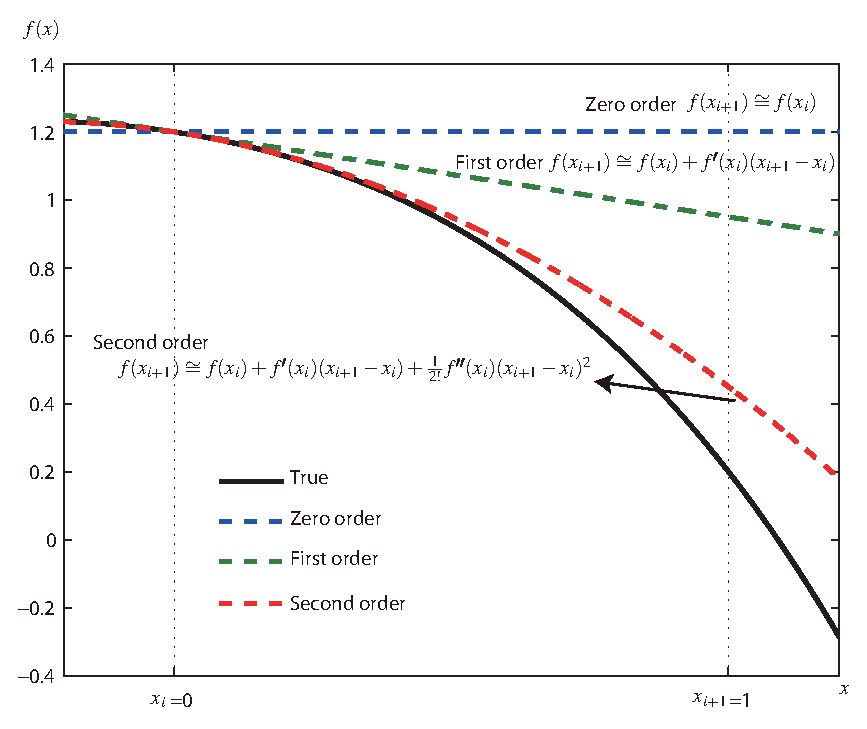
\includegraphics[keepaspectratio=true,width=0.8\linewidth]{figs/4-1.eps}
\caption{0차, 1차, 2차 Taylor 급수전개를 이용한 $x=1$에서의 함수 $f(x)=-0.1x^4-0.15x^3-0.5x^2-0.25x+1.2$의 근사}
\label{fig:4-1}
\end{figure}

\framebox{해}
함수의 형태를 알 고 있으므로, $f(0)=1.2$로부터 시작하고 $f(1)=0.2$의 값을 얻는다. 따라서 예측하고자 하는 참값은 $0.2$가 된다.\\
\textbf{zero-order}\\
$n=0$인 경우 Taylor 급수 근사
\begin{displaymath}
f\left(x_{i+1}\right) \cong 1.2
\end{displaymath}
즉, $f(1)\cong 1.2$가 된다. 절단오차를 계산하면 $x=1$에서
\begin{displaymath}
E_{t}=0.2-1.2=-1.0
\end{displaymath}
\textbf{first order}\\
$n=1$인 경우, $x=0$에서의 1차 도함수를 구하면,
\begin{eqnarray*}
f'(x)&=&-0.4x^3-0.45x^2-1.0x-0.25\\
f'(0)&=&-0.25
\end{eqnarray*}

따라서 1차 근사식은
\begin{displaymath}
f\left(x_{i+1}\right) \cong 1.2-0.25h
\end{displaymath}
즉, $f(1)\cong 0.95$가 된다. 절단오차를 계산하면 $x=1$에서
\begin{displaymath}
E_{t}=0.2-0.95=-0.75
\end{displaymath}
\textbf{second order}\\
$n=2$인 경우, $x=0$에서의 2차 도함수를 구하면,
\begin{eqnarray*}
f''(x)&=&-1.2x^2-0.9x-1.0\\
f''(0)&=&-1.0
\end{eqnarray*}

따라서 2차도함수값에 $1/2!$를 곱하여 추가한 2차 근사식은
\begin{displaymath}
f\left(x_{i+1}\right) \cong 1.2-0.25h-0.5h^2
\end{displaymath}
즉, $f(1)\cong 0.45$가 된다. 절단오차를 계산하면 $x=1$에서
\begin{displaymath}
E_{t}=0.2-0.45=-0.25
\end{displaymath}
\textbf{third order}\\
$n=3$인 경우, $x=0$에서의 3차 도함수를 구하면,
\begin{eqnarray*}
f^{(3)}(x)&=&-2.4x-0.9\\
f^{(3)}(0)&=&-9.0
\end{eqnarray*}

따라서 3차도함수값에 $1/3!$를 곱하여 추가한 3차 근사식은
\begin{displaymath}
f\left(x_{i+1}\right) \cong 1.2-0.25h-0.5h^2-0.15h^3
\end{displaymath}
즉, $f(1)\cong 0.3$이 된다. 절단오차를 계산하면 $x=1$에서
\begin{displaymath}
E_{t}=0.2-0.3=-0.1
\end{displaymath}
\textbf{fourth order}\\
$n=4$인 경우, $x=0$에서의 4차 도함수를 구하면,
\begin{eqnarray*}
f^{(4)}(x)&=&-2.4\\
f^{(4)}(0)&=&-2.4
\end{eqnarray*}

따라서 4차도함수값에 $1/4!$를 곱하여 추가한 4차 근사식은
\begin{displaymath}
f\left(x_{i+1}\right) \cong 1.2-0.25h-0.5h^2-0.15h^3-0.1h^4
\end{displaymath}
즉, $f(1)\cong 0.2$이 된다. 절단오차를 계산하면 $x=1$에서
\begin{displaymath}
E_{t}=0.2-0.2=0
\end{displaymath}

이때 나머지항을 살펴보자.
\begin{displaymath}
R_{4}=\frac{f^{(5)}(\xi)}{5!}h^{5}=0
\end{displaymath}
이는 4차 다항식의 5차 미분항은 항상 0이 되기 때문에, 정확한 값을 얻을 수 있다.
\\ \rule{\textwidth}{0.1pt}
\subsection{Talyor 급수전개에서의 나머지 항}
많은 경우에서 Taylor 급수의 실용적 가치는, 단지 몇 개의 항들만을 포함시키는 것만으로도 참값에 충분히 근접한 결과(공학적 측면에서)를 얻을 수 있다는 것이다. \textbf{충분히 근접한}값을 얻기 위해 얼마나 많은 항들이 필요한 지에 대한 평가는, 급수의 나머지 항을 기초로 하여 결정된다. 

\begin{displaymath}
R_{n}=\frac{f^{(n+1)}(\xi)}{(n+1)!}h^{n+1}
\end{displaymath}

\begin{table}[!hb]
\begin{tabular}{|l|}
\hline
그러나 식(\ref{eq:4-8})를 찾으려면, $x_{i}$와 $x_{i+1}$사이에 놓인$\xi$를 알아야 하고, $f(x)$의 $(n+1)$차 도함수를 알아야하는데,\\
이것을 안다면 굳이 Taylor 급수전개를 할 필요가 없다. \framebox{모순}\\
\hline
\end{tabular}
\end{table}

$x_{i}=\pi/4$에서의 $f(x)$값을 이용하여, $x_{i+1}=\pi/3$에서의 $f(x)=\cos x$를 근사하기 위해 Taylor급수전개를 6차까지 수행하면, (여기서 $h=\pi/3-\pi/4$) \textbf{MATLAB 코드 ~\ref{ap:2}장 (\pageref{ap:2}페이지)}
\begin{table}[!hbt]
\centering
\begin{tabular}{cccr}
\hline
\textbf{Order $n$} & $f^{(n)}(x)$ & $f(\pi/3)$ & $E_{t}$\\
\hline
0 & $\cos x$ & 0.707106781 & $-41.4$\\
1 & $-\sin x$ & 0.521986659 & $-4.4$\\
2 & $-\cos x$ & 0.497754491 & $0.449$\\
3 & $\sin x$ & 0.499869147 & $2.62\times10^{-2}$\\
4 & $\cos x$ & 0.500007551 & $-1.51\times10^{-3}$\\
5 & $-\sin x$ & 0.500000304 & $-6.08\times10^{-5}$\\
6 & $-\cos x$ & 0.499999988 & $2.44\times10^{-6}$\\
\hline
\end{tabular}
\end{table}

\clearpage
\subsection{수치미분}\label{sec:4-diff}
Taylor급수전개 식(\ref{eq:4-7})에서 $x$를 시간함수로 생각해보면,
\begin{equation}
f(t_{i+1})=f(t_{i})+f'(t_{i})(t_{i+1}-t_{i})+\frac{f''(t_{i})}{2!}(t_{i+1}-t_{i})^2+\frac{f^{(3)}(t_{i})}{3!}(t_{i+1}-t_{i})^3 +\cdots +\frac{f^{(n)}}{n!}(t_{i+1}-t_{i})^n+R_{n}
\end{equation}
1차 도함수의 항 뒤에 있는 모든 항을 $R_{1}$로 표현하면 다음과 같다.
\begin{equation}
f(t_{i+1})=f(t_{i})+f'(t_{i})(t_{i+1}-t_{i})+R_{1}
\label{eq:4-13}
\end{equation}
따라서 식(\ref{eq:4-13})을 사용하여 다음 도함수의 근사식을 구할 수 있다.
\begin{equation}
\star f'(t_{i})=\frac{f(t_{i+1})-f(t_{i})}{t_{i+1}-t_{i}}-\frac{R_{1}}{t_{i+1}-t_{i}}
\label{eq:4-14}
\end{equation}
Tayler급수의 절단오차 $R_{1}$은 식(\ref{eq:4-8})에 의해,
\begin{equation}
R_{1}=\frac{f''(\xi)}{2!}\left(t_{i+1}-t_{i}\right)^{2}
\end{equation}
따라서, 수치미분의 절단오차를 추정값은,
\begin{eqnarray}
\frac{R_{1}}{t_{i+1}-t_{i}}&=&\frac{f''(\xi)}{2!}\left(t_{i+1}-t_{i}\right)\\
&=&O\left(t_{i+1}-t_{i}\right)
\end{eqnarray}
즉, 절단오차는 시간간격에 비례하게 된다.

식(\ref{eq:4-14})는 수치해법에서 \textbf{유한제차분(finite divided difference)}이라고 불린다. 일반적으로 표현하면,
\begin{eqnarray}
f'(x_{i})&=&\frac{f(x_{i+1})-f(x_{i})}{x_{i+1}-x_{i}}+O\left(x_{i+1}-x_{i}\right)\\
&=&\frac{\Delta f_{i}}{h}+O(h)
\end{eqnarray}

\clearpage
\subsubsection{1차 도함수의 전진차분 근사}

여기서, $\Delta f_{i}$는 \textbf{전진차분(first forward difference)}이고, $h$는 구간 간격의 크기. 즉 근사값이 구해지는 구간의 길이이다.
$h$를 구간의 크기(절대값)로 표시되기 때문에 $i$를 시작으로 $i+1$에 도달하게 된다. 전체 항 $\Delta f/h$는 \textbf{1차 유한제차분(first finite divided difference)}라고 한다.
\begin{figure}[!hbpt]
\centering
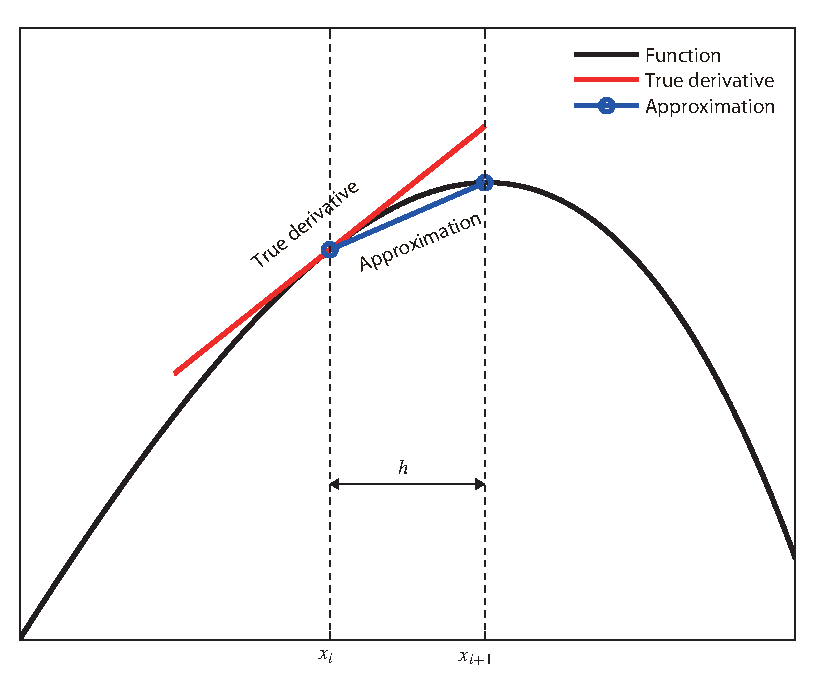
\includegraphics[keepaspectratio=true,width=0.5\linewidth]{figs/forward-deriv.eps}
\caption{전진 유한제차분 근사}
\label{fig:4-4a}
\end{figure}


\subsubsection{1차 도함수의 후진차분 근사}

현재 위치에서의 값을 기초로 하여 이전 값을 계산하기 위해 Taylor 급수를 다음과 같이 후진전개(backward expansion)한다.
\begin{equation}
f(x_{i-1})=f(x_i)-f'(x_i)h+\frac{f''(x_{i})}{2!}h^2-\cdots
\label{eq:4-19}
\end{equation}
1차 도함수 이상의 항들을 절단하고, 이를 재배열하면,
\begin{equation}\label{eq:4-backward}
f'(x_i) \cong \frac{f(x_i)-f(x_{i-1})}{h}= \frac{\nabla f_1}{h}
\end{equation}
여기서 오차는 $O(h)$이고 $\nabla f_1$는 \textbf{1차 후진차분(backward difference)}라고 한다.

\begin{figure}[!hbpt]
\centering
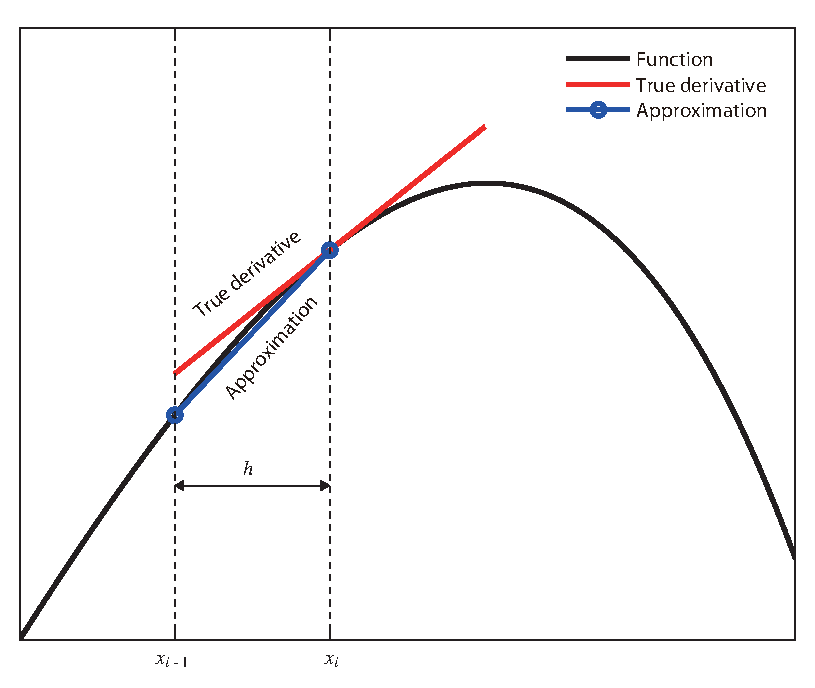
\includegraphics[keepaspectratio=true,width=0.5\linewidth]{figs/backward-deriv.eps}
\caption{후진 유한제차분 근사}
\label{fig:4-4b}
\end{figure}

\subsubsection{1차 도함수의 중심차분 근사}
1차 도함수를 근사적으로 구하기 위한 세번째 방법은 다음과 같이 주어진
\begin{equation}
f(x_{i+1})=f(x_i)+f'(x_i)h+\frac{f''(x_i)}{2!}h^2+\cdots
\label{eq:4-21}
\end{equation}
전진 Taylor 급수전개에서 식(\ref{eq:4-19})를 뺌으로써 얻을 수 있다.
\begin{equation}
f(x_{i+1})=f(x_{i-1})+2f'(x_i)h+\frac{2f^{(3)}(x_i)}{3!}h^3+\cdots
\end{equation}
이를 $f'(x_{i+1})$에 대해 정리하면
\begin{eqnarray}
f'(x_i)&=&\frac{f(x_{i+1})-f(x_{i-1})}{2h}-\frac{f^{(3)}(x_i)}{6}h^2-\cdots\\
&=&\frac{f(x_{i+1})-f(x_{i-1})}{2h}-O(h^2)
\label{eq:4-22}
\end{eqnarray}
식(\ref{eq:4-22})는 1차 도함수에 대한 중심차분(centered difference)의 표현이다. 절단오차의 경우. $O(h)$인 전진 또는 후진차분과는 달리 $O(h^2)$가 된다. 따라서 중심차분이 수치미분값을 나타내는데 더 정확한 표현이라는 것을 나타내준다.
\begin{figure}[!hbpt]
\centering
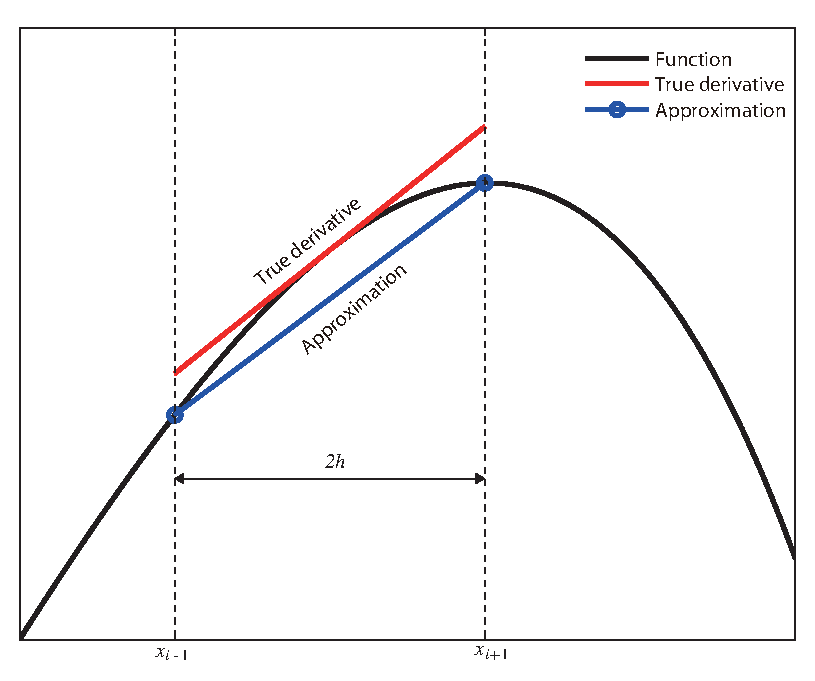
\includegraphics[keepaspectratio=true,width=0.5\linewidth]{figs/centered-deriv.eps}
\caption{중심 유한제차분 근사}
\label{fig:4-4c}
\end{figure}

\clearpage
\subsubsection{고차 도함수의 유한차분근사}
Taylor 급수전개를 사용하여 고차 도함수의 수치적 근사식을 유도할 수 있다. $f(x_{i+2})$를 위한 Taylor 급수전개를 $f(x_{i})$을 기준으로 수행하면,
\begin{equation}
f\left(x_{i+2}\right) = f(x_{i})+f'(x_{i})(2h)+\frac{f''(x_{i})}{2!}(2h)^2 + \cdots
\label{eq:4-23}
\end{equation}
식(\ref{eq:4-21})에 2를 곱한후, 식(\ref{eq:4-23})에서 빼면,
\begin{equation}
f(x_{i+2})-2f(x_{i+1})=-f(x_{i})+f''(x_{i})h^2 + \cdots
\end{equation}
즉 함수 $f(x)$에 대하여 $x_{i}$에서의 2차도함수는
\begin{equation}
f''(x_i)=\frac{f(x_{i+2})-2f(x_{i+1})+f(x_i)}{h^2}+O(h)
\end{equation}
이 관계식은 \textbf{2차 전진유한제차분(second forward finite divided difference)}이라고 한다. 비슷한 과정을 통해 다음과 같은 후진차분식과,
\begin{equation}
f''(x_i)=\frac{f(x_{i})-2f(x_{i-1})+f(x_{i-2})}{h^2}+O(h)
\end{equation}
다음의 중심차분식을 얻을 수 있다.
\begin{equation}
f''(x_i)=\frac{f(x_{i+1})-2f(x_i)+f(x_{i-1})}{h^2}+O(h^2)
\end{equation}

1차 유한제차분식 처럼 절단오차의 Big-O notation $O(h^2)$으로 쓰기때문에 2차도함수의 중심차분근사가 더 정확한 결과를 얻는다.

\subsection{오차의 전파}
근사값에 의해 함수값들의 오차가 어떻게 전파되는지 파악하기 위해 오차의 전파를 해석해야 한다.
\subsubsection{단일 변수 함수}
단일 독립변수 $x$의 함수 $f(x)$가 있다고 가정하자. $\tilde{x}$가 $x$의 근사값이라고 가정할 때, $x$와 $\tilde{x}$의 오차가 함수값에 미치는 영향을 구해보자.

\begin{equation}
\Delta f(\tilde{x})=\left|f(x)-f(\tilde{x})\right|
\end{equation}
$\Delta f(\tilde{x})$의 값을 구하기 위한 문제는 $x$를 모르기 때문에 $f(x)$를 알 수 없는 문제가 있다 하지만, $\tilde{x}$가 $x$에 매우 가깝고, $f(\tilde{x})$가 연속이며 미분가능하면 Taylor급수 전개($f(\tilde{x})$에 인접한 $f(x)$)를 통해 함수값의 오차를 계산할 수 있다.

\begin{equation}
f(x)=f(\tilde{x})+f'(\tilde{x})(x-\tilde{x})+\frac{f''(\tilde{x})}{2!}(x-\tilde{x})^2+ \cdots
\end{equation}
2차와 그 이상의 고차항들을 절단하고 결과를 재배열하면,
\begin{equation}
f(x)-f(\tilde{x})\cong f'(\tilde{x})(x-\tilde{x})
\end{equation}
또는
\begin{equation}
\Delta f(\tilde{x})=\left|f'(\tilde{x})\right| \Delta \tilde{x}
\label{eq:4-25}
\end{equation}
여기서, $\Delta f(\tilde{x})=\left|f(x)-f(\tilde{x})\right|$는 함수의 추정오차이며, $\Delta \tilde{x}=\left|x-\tilde{x}\right|$는 $x$에 대한 오차의 추정값이다. 식(\ref{eq:4-25})는 함수의 도함수 및 독립변수의 추정오차값이 주어진 경우, $f(x)$의 오차의 근사값을 계산할 수 있도록 해준다.

\subsubsection{다중 변수 함수}
같은 방식으로 독립변수가 1개 이상의 경우의 함수에도 일반화될 수 있다. 즉, Taylor급수의 다중 변수 형태를 사용하여 얻을 수 있다. 함수가 두 개의 독립변수 $u$와 $v$의 함수라면, Taylor 급수는 다음과 같이 쓸 수 있다.

\begin{equation}
\begin{split}
f(u_{i+1},v_{i+1})=&f(u_i ,v_i)+\frac{\partial f}{\partial u}(u_{i+1}-u_{i})+\frac{\partial f}{\partial v}(v_{i+1}-v_{i})\\
&+\frac{1}{2!}\left[\frac{\partial^2 f}{\partial{u^2}}(u_{i+1}-u_{i})^2+2\frac{\partial^2 f}{\partial u \partial v}(u_{i+1}-u_{i})(v_{i+1}-v_{i})+\frac{\partial^2 f}{\partial v^2}(v_{i+1}-v_{i})^2\right]+\cdot
\end{split}
\label{eq:4-26}
\end{equation}
여기서 모든 편도함수들을 기준점 $i$에서 구한다. 만일 2차와 그 이상의 고차 항들을 버리면, 식(\ref{eq:4-26})은 다음의 식으로 풀 수 있다.
\begin{equation}
\Delta f(\tilde{u},\tilde{v})=\left|\frac{\partial f}{\partial u}\right|\Delta \tilde{u}+\left|\frac{\partial f}{\partial v}\right|\Delta \tilde{v}
\end{equation}
여기서 $\Delta\tilde{u}$와 $\Delta\tilde{v}$는 각각 $u$와 $v$의 추정오차값이다.
$n$개의 독립변수, $\tilde{x}_{1},\tilde{x}_{2},\cdots,\tilde{x}_{n}$가 $\Delta\tilde{x}_{1},\Delta\tilde{x}_{2},\cdots,\Delta\tilde{x}_{n}$의 오차를 갖는다면, 다음과 같은 일반적인 관계식으로 쓸 수 있다.
\begin{equation}
\Delta f(\tilde{x}_{1},\tilde{x}_{2},\cdots,\tilde{x}_{n})\cong \left|\frac{\partial f}{\partial x_{1}}\right| \Delta\tilde{x}_{1}+\left|\frac{\partial f}{\partial x_{2}}\right| \Delta\tilde{x}_{2}+\cdots+\left|\frac{\partial f}{\partial x_{n}}\right| \Delta\tilde{x}_{n}
\label{eq:4-27}
\end{equation}
\\
\framebox{예제} \textbf{다중 변수 함수에서의 오차의 전파}\\
\rule{\textwidth}{0.1pt}
배의 돛대의 위 끝에서의 휨(deflection) $y$는 다음과 같다.
\begin{displaymath}
y=\frac{FL^4}{8EI}
\end{displaymath}
여기서 $F$는 균일한 측면 하중($N/m$), $L$은 높이($m$), E는 탄성계수($N/m^2$), $I$는 관성모멘트($m^4$)이다. 다음의 데이터를 사용하여, $y$의 오차를 추측하라.

\begin{align*}
\tilde{F}&=750N/m &
 \Delta\tilde{F}&=30N/m\\
\tilde{L}&=9m &
 \Delta\tilde{L}&=0.03m \\
\tilde{E}&=7.5\times 10^{9}N/m^2 &
 \Delta\tilde{E}&=5 \times 10^{7}N/m^2\\
\tilde{I}&=0.0005m^4 &
 \Delta\tilde{I}&=0.000005m^4
\end{align*}
\\
\framebox{해}
원래 휨식에 측정값을 대입하여 구한 근사값은,
\begin{align*}
\tilde{y}&=\frac{750 \times 9^4}{8 \times (7.5\times10^9) \times 0.0005}\\
&=1.64025\times 10^{-1}
\end{align*}

추정된 변형의 오차를 구하기 위해, 식(\ref{eq:4-27})을 사용하면,
\begin{align*}
\Delta y(\tilde{F},\tilde{L},\tilde{E},\tilde{I}) &=\left|\frac{\partial y}{\partial F}\right| \Delta\tilde{F}+\left|\frac{\partial y}{\partial L}\right| \Delta\tilde{L}+\left|\frac{\partial y}{\partial E}\right| \Delta\tilde{E}+\left|\frac{\partial y}{\partial I}\right| \Delta\tilde{I}\\
\Delta y(\tilde{F},\tilde{L},\tilde{E},\tilde{I}) &\cong \frac{\tilde{L}^4}{8\tilde{E}\tilde{I}}\Delta\tilde{F} + \frac{\tilde{F}\tilde{L}^3}{2\tilde{E}\tilde{I}}\Delta{L} + \frac{\tilde{F}\tilde{L}^4}{8\tilde{E}^2\tilde{I}}\Delta\tilde{E} + \frac{\tilde{F}\tilde{L}^4}{8\tilde{E}\tilde{I}^2}\Delta\tilde{I}
\end{align*}

값을 대입하여 추정된 오차를 구하면
\begin{equation*}
\Delta y=0.006561+0.002187+0.001094+0.00164=0.011482
\end{equation*}
즉, $y = 0.164025 \pm 0.011482$의 결과가 나온다. $y$의 최소값은 $0.152543$, $y$의 최대값은 $0.175507$라고 추정할 수 있는데, 이 값이 타당한지 알아보기 위해 변형식의 분자에 최대값들을 대입하고 분모에 최소값들을 대입하여 최대값 $y_{\max}$와 분자에 최소값들을 대입하고 분모에 최대값들을 대입하여 최소값 $y_{\min}$을 찾아보면
\begin{align*}
y_{\min}&=\frac{720 \times 8.97^4}{8 \times (7.55 \times 10^9) \times 0.000505} = 0.152818\\
y_{\max}&=\frac{780 \times 9.03^4}{8 \times (7.45 \times 10^9) \times 0.000495} = 0.175790
\end{align*}

휨변형에 대한 오차영향 검토
\begin{align*}
\Delta y(\tilde{F},\tilde{L},\tilde{E},\tilde{I}) &\cong \frac{\tilde{L}^4}{8\tilde{E}\tilde{I}}\Delta\tilde{F} + \frac{\tilde{F}\tilde{L}^3}{2\tilde{E}\tilde{I}}\Delta{L} + \frac{\tilde{F}\tilde{L}^4}{8\tilde{E}^2\tilde{I}}\Delta\tilde{E} + \frac{\tilde{F}\tilde{L}^4}{8\tilde{E}\tilde{I}^2}\Delta\tilde{I}\\
&=2.187\times 10^{-4} \Delta\tilde{F} + 7.29\times 10^{-2} \Delta\tilde{L} + 2.187\times 10^{-11} \Delta\tilde{E} + 3.2805\times10^{2} \Delta\tilde{I}
\end{align*}
\rule{\textwidth}{0.1pt}

\subsubsection{안정성과 조건수}
대체적으로 수학문제의 조건(condition)은 입력값의 변화에 대한 민감도와 관련되어 있다. 입력값의 불확실성이 수치해법에 의해 크게 확대되면 계산이 \textbf{수치적으로 불안정}(numerically unstable)하다고 말한다. 함수$f(x)$의 오차를 1차 Taylor급수로 확인해보자.
\begin{equation}
f(x)=f(\tilde{x})+f'(\tilde{x})(x-\tilde{x})
\end{equation}
위의 식을 함수값$f(x)$의 상대오차를 구하기위해 변형하면
\begin{equation}
\epsilon_{f}=\frac{f(x)-f(\tilde{x})}{f(x)}\cong\frac{f'(\tilde{x})(x-\tilde{x})}{f(\tilde{x})}
\end{equation}
$x$의 상대오차는 $\epsilon_{x}=(x-\tilde{x})/\tilde{x}$이고, \textbf{조건수}(condition number)\footnote{\url{http://en.wikipedia.org/wiki/Condition_number}}는 이들 상대오차의 비로 정의 된다.
\begin{equation}
\kappa=\frac{\epsilon_{f}}{\epsilon_{x}}=\frac{\tilde{x}f'(\tilde{x})}{f(\tilde{x})}
\end{equation}
이 조건수는 $x$의 불확실성이 함수값$f(x)$에 얼마나 영향을 미치는지에 대한 척도를 제공한다.

수치해석 분야에서 함수의 조건수(condition number)는 argument에서 의 작은 변화의 비율에 대해 함수가 얼마나 변화할 수 있는지에 대한 argument measure이다. 여기서 "함수"는 문제의 해를 의미하며, "argument"는 문제에서의 데이터를 의미한다. 작은 조건수를 갖는 문제를 "well-conditioned"라고 하며, 큰 조건수를 갖는 문제를 "ill-conditioned"라고 한다. 조건수는 문제의 고유한 성질이다.

\clearpage
\framebox[1.1\width]{과제2 (제출기한 10월9일)}\\
1. $\cos x$의 Maclaurin 급수는 다음과 같이 주어진다.
\begin{eqnarray*}
\cos x&=&\sum_{n=0}^{\infty}\frac{(-1)^n}{(2n)!}x^{2n}\\
&=&1-\frac{x^2}{2!}+\frac{x^4}{4!}-\frac{x^6}{6!}+\frac{x^8}{8!}-\cdots
\end{eqnarray*}
가장 간단한 형태인 $\cos x =1$로부터 시작하여 항들을 추가해 가면서 $\cos(\pi/3)$의 값을 구하라. 각각의 항이 추가될 때마다, 절단오차(상대오차)를 계산하라.\\
2. $x\in \mathbb{R}$에 대하여 $|x|>1$의 개구간 미분이 가능한 다음 함수$f(x)$의 Taylor 급수를 전개하고, $x=3$에서 5차 근사값을 구하고, 절단오차 $E_{t}$를 각각의 차수에 대하여 표시하라.
\begin{displaymath}
f(x)=\frac{x}{x-1}
\end{displaymath}
3. 다음 함수 $f(x)=\ln(\cos x), x\in (-\pi/2,\pi/2)$를 7차이상의 다항식으로 전개하라\\

참고 Maclaurin 급수
\begin{eqnarray*}
\ln(1-x)&=&-\sum_{n=1}^{\infty}\frac{x^n}{n}, (|x|\leq 1, x\neq 1)\\
\ln(1+x)&=&\sum_{n=1}^{\infty}(-1)^{n+1}\frac{x^n}{n}, (|x|\leq 1, x\neq -1)
\end{eqnarray*}
4. 정확도(accuracy)와 정밀도(precision)에 대하여 조사하라\footnote{\url{http://en.wikipedia.org/wiki/Accuracy_and_precision}} 그리고 각 전공영역에 맞추어  특정한 공학적 이슈를 예를들어 불확실성(uncertainty)에 대하여 자신의 생각을 쓰시오.
